\documentclass{TDP003mall}



\newcommand{\version}{Version 1.1}
\author{Nils Bark, \url{nilba048@student.liu.se}\\
  Hadi Ansari, \url{hadan326@student.liu.se}}
\title{Dokumentmall}
\date{2020-12-16}
\rhead{Nils Bark\\
Hadi Ansari}



\begin{document}
\projectpage
\section{Revisionshistorik}
\begin{table}[!h]
\begin{tabularx}{\linewidth}{|l|X|l|}
\hline
Ver. & Revisionsbeskrivning & Datum \\\hline
0.1 & Första utkast skapat & 2020-11-27\\\hline
1.0 & Uppdatering av utkast enligt feedback från handledare & 2020-12-07\\\hline
1.1 & Sista uppdatering inför inlämning & 2020-12-16\\\hline
\end{tabularx}
\end{table}

\section{Beskrivning av Entity}
Nedan kommer en lista över alla funktioner och variabler som finns i klassen \texttt{Entity}.
\subsection{Variabler}
\begin{itemize}
\item \texttt{sf::Vector2f location}: Innehåller två koordinater av typen float som representerar spelarens position på spelplanen.
\item \texttt{sf::Sprite sprite}: Fungerar som figurens kropp och kan täckas av en textur.
\item \texttt{float speed}: Används för att bestämma objekts hastighet. 
\item \texttt{int health}: Bestämmer objektets livspoäng.
\item \texttt{int width och int height}: Bestämmer objektets storlek.
\end{itemize}


\subsection{Funktioner}
\begin{itemize}
\item \texttt{virtual void Tick(sf::Time const \& delta, World \& world)}: Uppdaterar objektens beteende. 
Den implementeras av de härledda klasserna och beteer sig där på olika sätt. 
Till exempel för Big plane så subtraheras x-koordinaten med ett värde som är bundet till hastigheten och tiden som har gått sedan förra uppdateringen.
\item \texttt{virtual void render(sf::RenderWindow \&window) = 0}: Ritar ut spelobjektet på skärmen.
\item \texttt{bool kill\_me()}: Kontrollerar om ett objekt ska förstöras (till exempel om det befinner sig utanför spelplanen) och returnerar true om så är fallet.
\item \texttt{virtual void collision(vector<entity*> objects, World \& world) = 0}: Tar en lista som inehåller entity-pekare till alla andra spelobjekt, 
utöver det som kallat på funktionen, och kontrollerar vilket av  dem objektet har kolliderat med. 
Har flera olika effekter beroende på vilket objekt som har kolliderat med ett annat. 
Till exempel förlorar spelaren liv om den kolliderar med en fiende. 
\item \texttt{virtual string get\_type() = 0}: Returnerar objektets typ i form av en sträng.
\item \texttt{virtual sf::Sprite get\_sprite() const}: Returnerar objektets sprite.
\item \texttt{int get\_health() const}: Returnerar objektets liv.
\item \texttt{virtual void freeze()}: Pausar alla spelets timers när spelet går till \texttt{pause\_state}.

\end{itemize}

\texttt{Entity} är en \texttt{abstract class} som alla understående klasser i spelet ärver ifrån. 
Detta innebär att alla dess variabler och funktioner är tillgängliga direkt i de härledda klasserna.
\texttt{Entity} låter oss därmed uppdatera alla andra objekt i spelet. 
Detta sker via funktionen \texttt{tick()} som tar och uppdaterar positionen för alla objekt på skärmen plus andra beteenden beroende på objektet. 
\texttt{Tick()} är en \texttt{virtual} funktion som kan överskrivas i de härledda klasserna.
Tack vare tidsberäkningen som sker inuti funktionen är vi oberoende av spelets bildfrekvens och tiden det tar att hantera alla händelser i loopen.
Alla datamedlemmar förutom \texttt{location} i basklassen kommer att initieras av de härledda klassernas constructor. 
till exempel kommer spelarens \texttt{speed} att initieras när spelaren skapas och inte innan.
Exempel på extra beteenden som uppdateras av tick (utöver uppdatering av position) är till exempel att \texttt{Big\_Plane} kan lägga till en \texttt{enemy\_bullet} på spelplanen

\section{Beskrivning av Player}
Nedan kommer en lista över alla funktioner och variabler som finns i klassen \texttt{Player}.
\subsection{Variabler}
\begin{itemize}
\item \texttt{float shoot\_speed}: Bestämmer tiden som måste passera efter att spelaren har skjutit innan den får skjuta igen.
\item \texttt{sf::Clock shoot\_timer}: Mäter tiden som sen kontrolleras mot \texttt{shoot\_speed}.
\item \texttt{sf::Time shoot\_time}: Sparar tiden från \texttt{shoot\_timer}.
\item \texttt{bool shield}: Är true om spelaren har shield-effekten aktiv.
\item \texttt{sf::Clock shield\_timer}: Räknar tiden från och med att spelaren plockade upp en shield-powerup
\item \texttt{sf::Time shield\_time}: Sparar tiden från \texttt{shield\_timer}.
\item \texttt{bool tripleshot}: Indikerar om spelaren har en triple-shot powerup aktiv.
\item \texttt{sf::Clock triple\_timer}: Räknar tiden från och med att spelaren plockade upp en tripleshot-powerup.
\item \texttt{sf::Time triple\_time}: Sparar tiden från \texttt{triple\_timer}.
\item \texttt{static bool invincible}: Indikerar om spelarens ödödlighetsperiod är aktiv.
\item \texttt{sf::Clock invincibility\_timer}: Räknar tiden från och med att spelarens odödlighetsperiod aktiverades:
\item \texttt{sf::Time invincibility\_time}: Sparar tiden från \texttt{invincibility\_timer}.
\item \texttt{bool give\_invincible}: Indikerar om spelaren ska ges sin odödlighetsperiod.
\item \texttt{bool freeze\_state}: Indikerar om spelet är pausat.
\end{itemize}

\subsection{Funktioner}
\begin{itemize}
\item \texttt{string get\_shield\_time()}: Returnerar den kvarstående tiden från \texttt{shield\_clock}.
\item \texttt{bool has\_shield()}: Returnerar true om spelaren har en shield aktiv, annars false.
\item \texttt{static bool is\_invincible()}: Kollar om spelaren är odödlig.
\item \texttt{void cheat()}: Kontrollerar om fusk ska aktiveras (via korrekt tangent).
\item \texttt{void set\_position()}: Uppdaterar spelarens position.
\item \texttt{void update\_status()}: Uppdaterar spelarens powerups. Till exempel om spelaren fortfarande ska ha dem aktiva.
\item \texttt{void shoot()}: Kontrollerar att spelaren tillåts skjuta, och gör i så fall det.
\end{itemize}

\texttt{Player} representerar det objekt som användaren kommer att ha kontroll över under spelets gång. 
Det är en härledd klass av \texttt{Textured\_object} (som i sin tur härleds från \texttt{Entity}) och ärver därmed alla datamedlemmar och funktioner därifrån. 
Den har också en känna-till-relation till \texttt{player\_bullet} och \texttt{Power-up}.
Player överskriver \texttt{tick()} för att kunna uppdatera sitt specifika beteende.
I spelarens konstruktor initieras spelarens alla datamedlemmar.
\texttt{tick()} returnerar alltid true när det går att uppdatera spelaren. Annars returnerar den false vilket indikerar att spelaren har förstörts.

Spelarens kollision med andra objekt kontrollerar ständigt under spelets gång via \texttt{collision()} från \texttt{entity}. 
Baserat på vilket objekt som spelaren kolliderar med kan flera olika saker hända.
Till exempel tar spelaren skada vid kollision med fiender (förutom då spelaren har en shield aktiv), medan den diverse aktiverar effekter vid kollision med power-ups. 
Den enda kollisionen som ignoreras av spelaren är med dess egna skott (och fienders skott ifall spelaren har en shield aktiv).



\section{Diskussion}
Flera olika för- och nackdelar har visat sig under projektets gång. Här kommer vi att nämna och diskutera några av de viktigaste vi har lagt märkte till. 
Först ut är \texttt{collision} som fungerar på ett mycket ineffektivt sätt. Den kontrollerar nämligen vid varje uppdatering om varje objekt har kolliderat med något annat objekt. 
Den kontrollerar då kollision mot alla andra objekt på spelplanen. Även om det första objektet som kontrolleras är det som kollideras med fortsätter den att gå igenom alla möjliga objekt. En fördel med vårt system är dock att det låter båda objekten i en kollision påverkas på olika sätt om till exempel båda objekten ska ta skada vid en kollision.

Det sker viss kodupprepning i vår \texttt{Enemy}-klass eftersom vi har seperata underklasser för varje fiendetyp. Här kunde vi istället ha designat spelet så att alla, eller åtminstånde de flesta, fiender kan skapas från samma klass. Dock togs detta problemet upp för sent för att kunna åtgärdas på ett tidseffektivt sätt. I nuläget gör denna design det dock lätt att lägga till fler fiendetyper, speciellt ifall de har nya egenskaper.

\section{Externa filformat} 
Vi skapade ett eget filformat .sw (som i praktiken är en enkel textfil) där vi sparar varje nivå. Texten i filen skrivs i formatet: [y-koordinat] [fiendenamn (eller None)]. 
Detta läses sedan in av programmet som då lägger in alla fiender på spelplanen samtidigt tills de når ett None (då tar det en paus på 2 sekunder). På så sätt kan man skapa vågor av fiender.
\begin{figure}[h!]
\centering
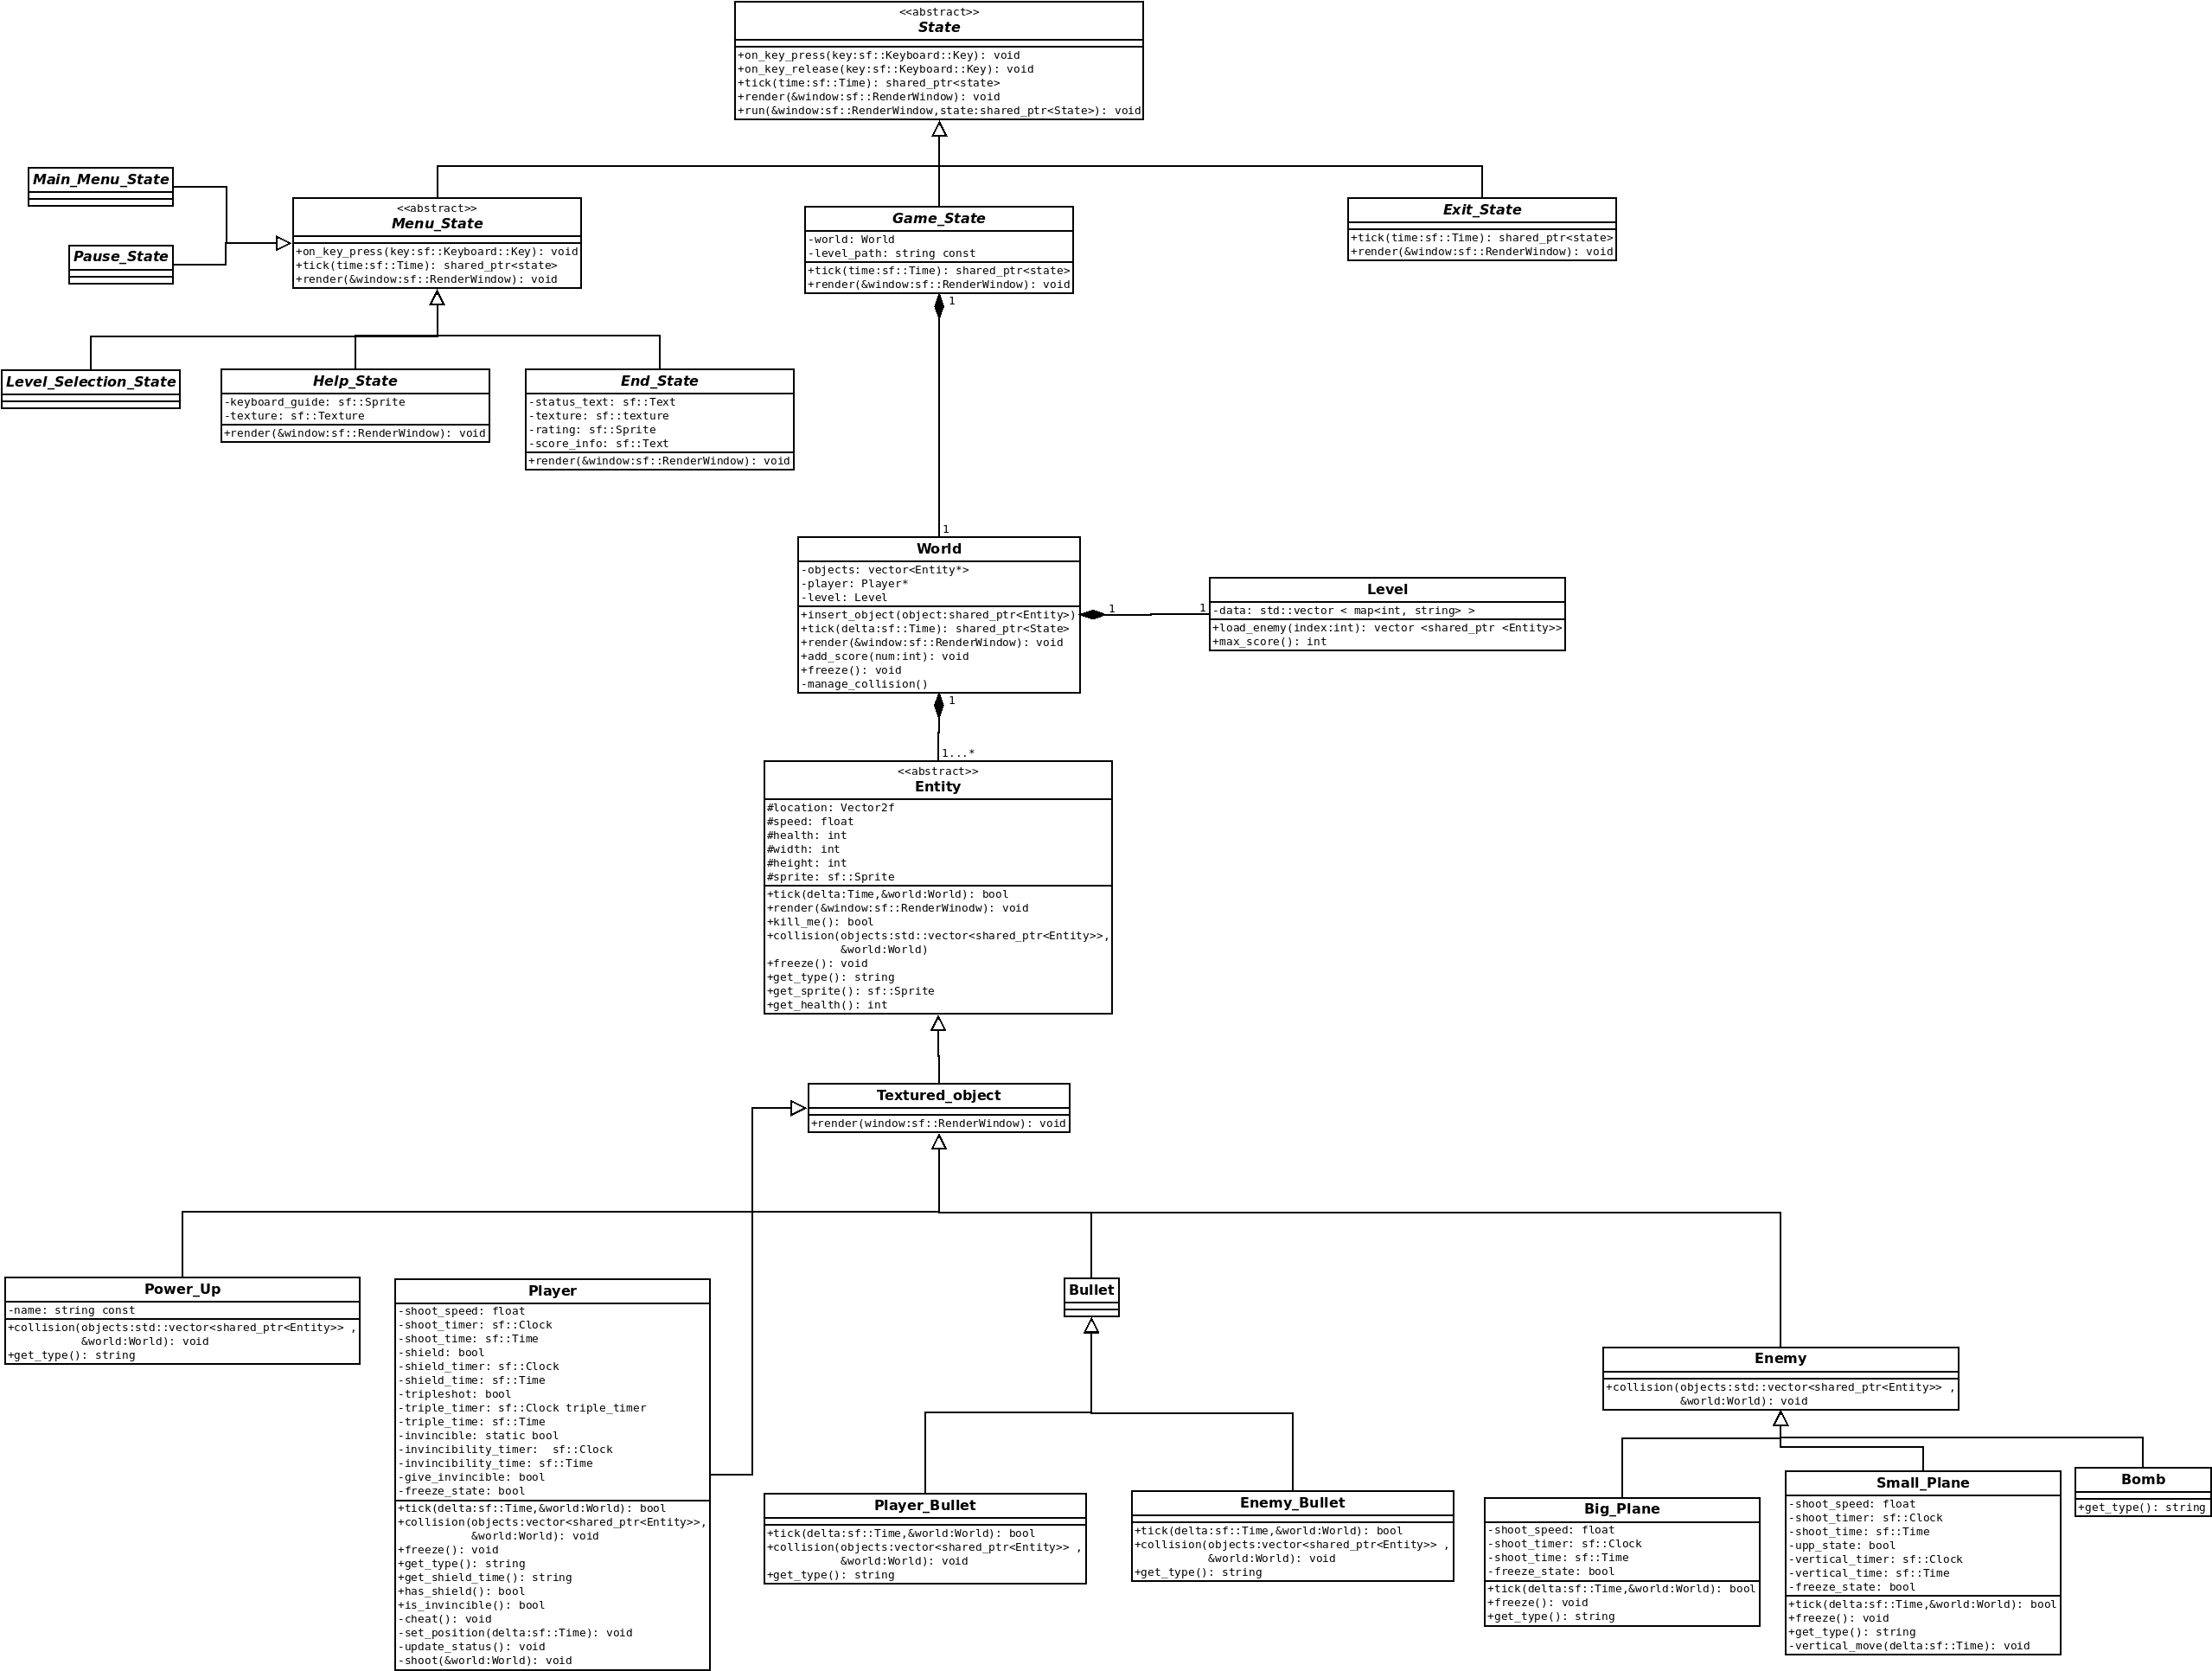
\includegraphics[scale=0.2]{UML_diagram.png}
\label{}
\caption{UML-diagram över spelet}
\end{figure}
\end{document}
